\documentclass{theozettel}

%%%%%%%%%%%%%%%%%%%%%%%%%%%%%%%%%%%%%%%%%%%%%%%%%%%%%%%%%%%%%%%%%%%%%%%%%%%%%%%%%%%%%%%%%%%%%%%%%%%%%%%%%%%%%%
% page geometry
%%%%%%%%%%%%%%%%%%%%%%%%%%%%%%%%%%%%%%%%%%%%%%%%%%%%%%%%%%%%%%%%%%%%%%%%%%%%%%%%%%%%%%%%%%%%%%%%%%%%%%%%%%%%%%
\geometry{
	left=20mm,
	right=20mm,
	top=25mm,
	bottom=20mm
}
%%%%%%%%%%%%%%%%%%%%%%%%%%%%%%%%%%%%%%%%%%%%%%%%%%%%%%%%%%%%%%%%%%%%%%%%%%%%%%%%%%%%%%%%%%%%%%%%%%%%%%%%%%%%%%

\pgfplotsset{compat=1.16}

%\renewcommand{\phi}{\varphi}

\usepackage{parskip}
\usepackage{dsfont}
\newcommand{\difd}{\text{d}}
\usepackage{titlesec} 
\titleformat{\section}[runin]
{\normalfont\large\bfseries}{\thesubsection}{1em}{}
\titleformat{\subsection}[runin]
  {\normalfont\normalsize\bfseries}{\thesubsubsection}{1em}{}
  
\renewcommand{\epsilon}{\varepsilon}
\newcommand{\vol}{\operatorname{vol}}

\theoI{8}

\begin{document}
\punkteV{8.1}{8.2}{8.3}{8.4}

\section*{Aufgabe 8.1} 

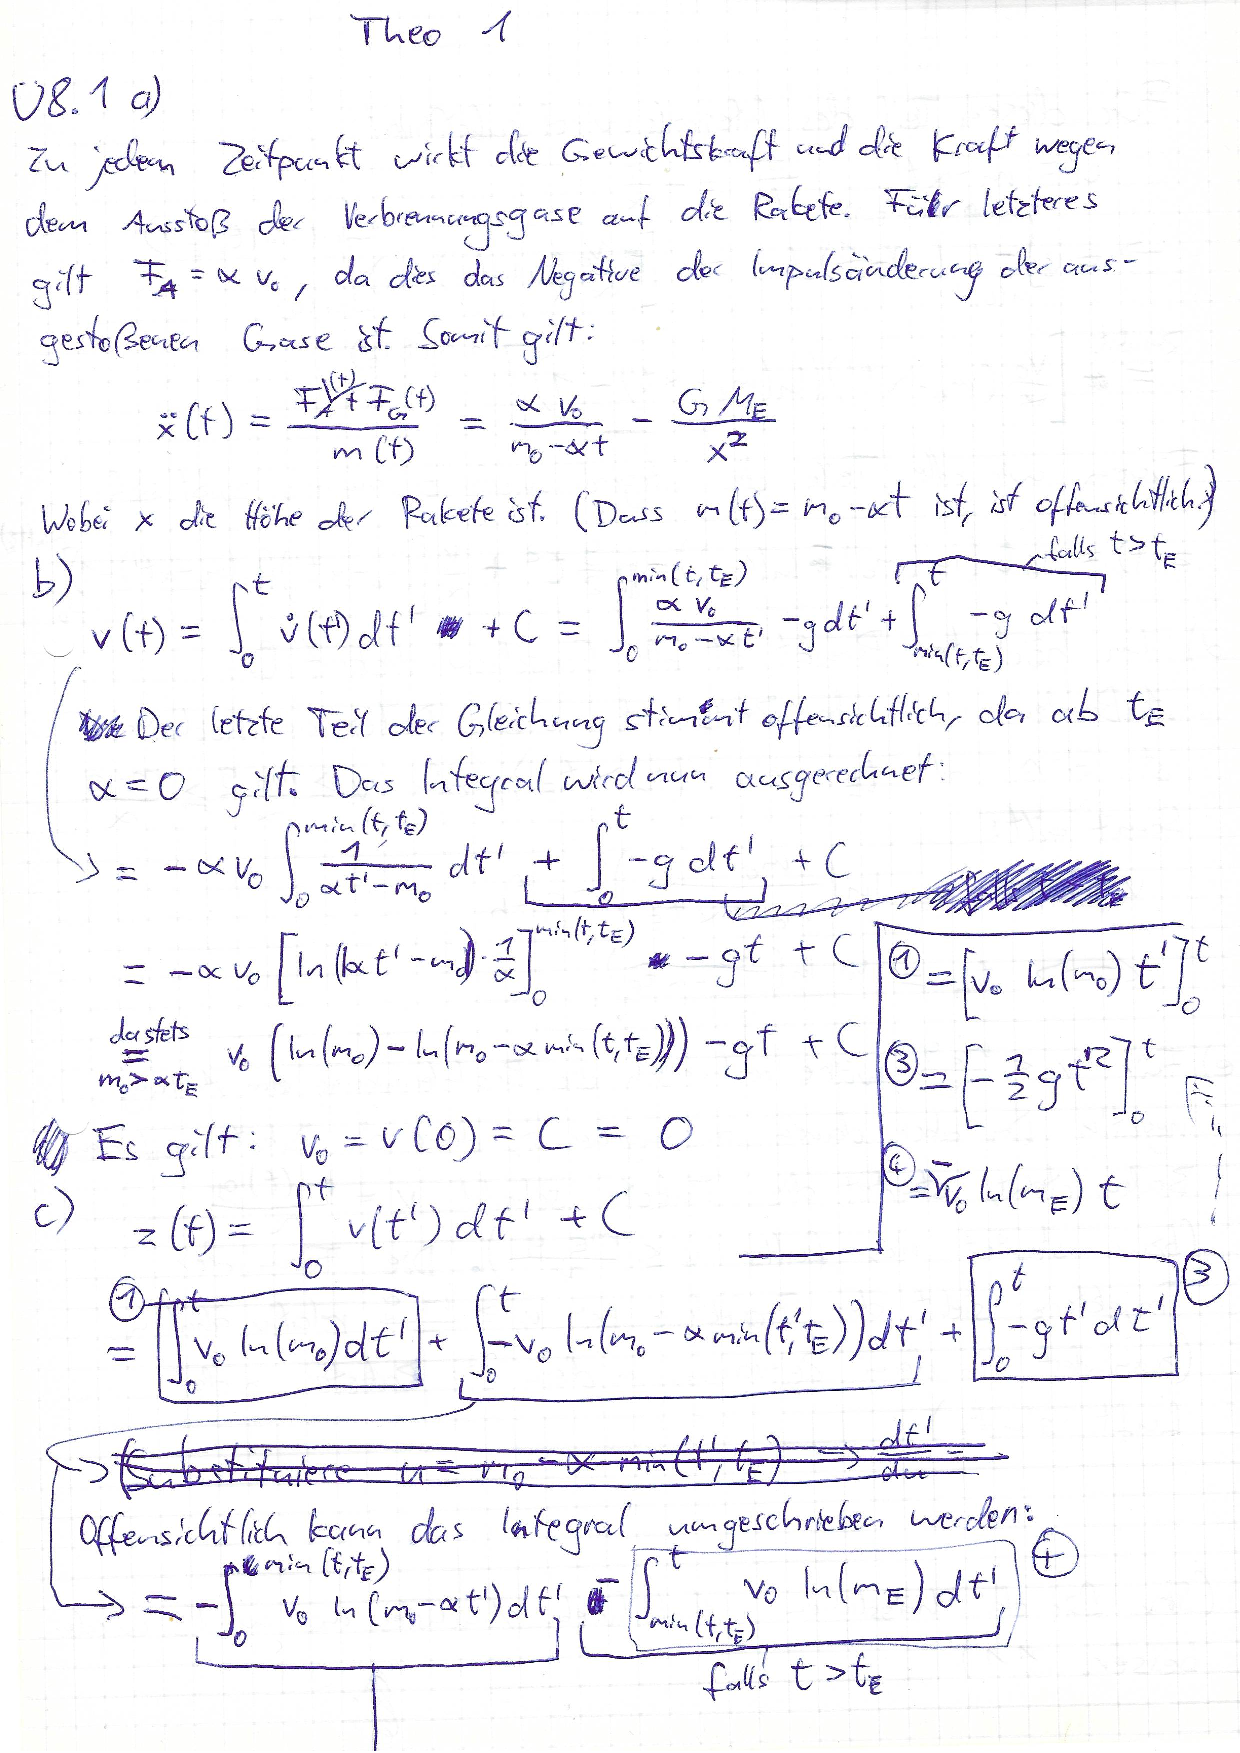
\includepdf[pages=-, pagecommand={\thispagestyle{plain}}]{Theo1U8A1.pdf}


\section*{Aufgabe 8.2}	
\begin{center}
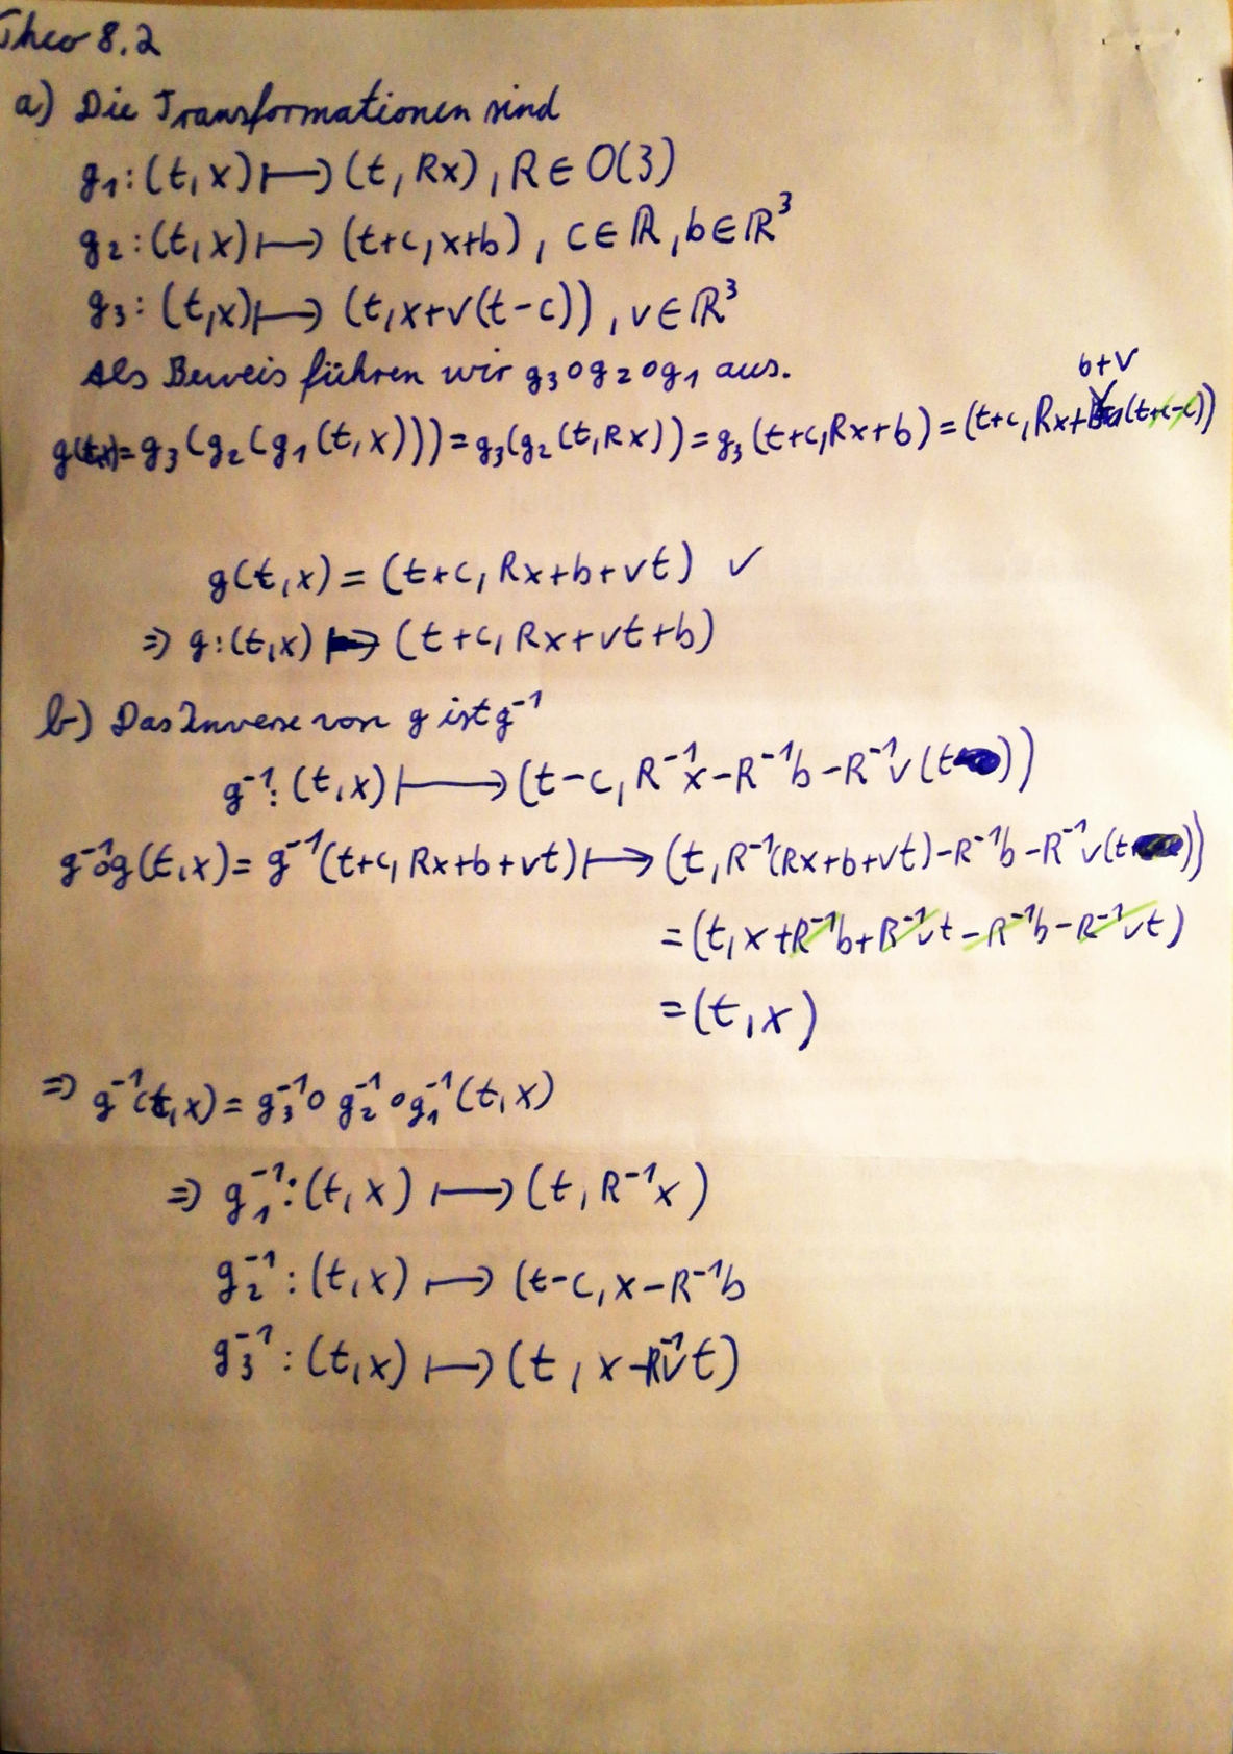
\includegraphics[width=14cm]{PTP8-2)_1.pdf}
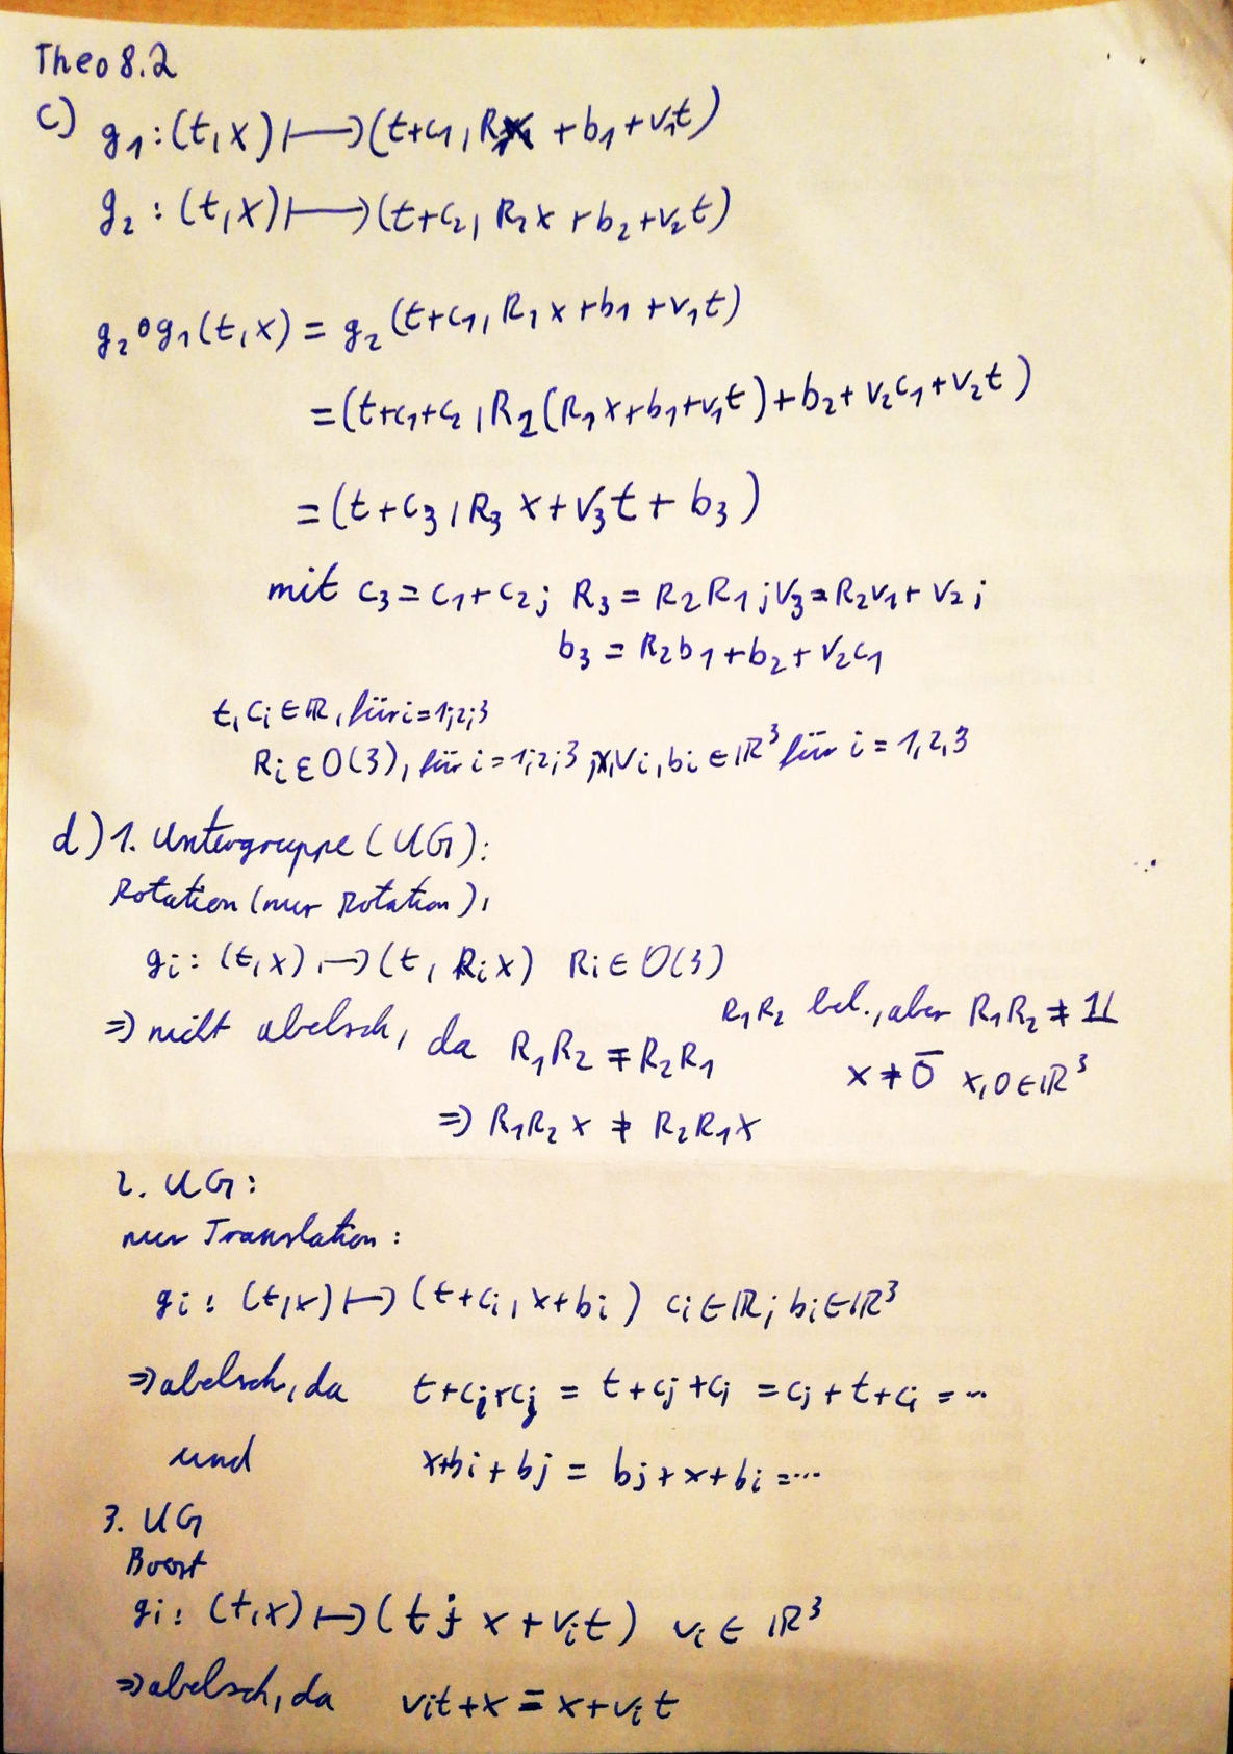
\includegraphics[width=14cm]{PTP8-2)_2.pdf}
\end{center}
\newpage



\section*{Aufgabe 8.3}
Jedes eindimensionale zeitunabhängige Kraftfeld ist konservativ, es gilt hier also:
	\[
		E = \frac{m}{2} \dot{x} + V(x) = \frac{m}{2}\dot{x} + A|x|^{n}.
	\]
Nun gilt es die Dauer einer Schwingung des Massepunkts vom Umkehrpunkt $x_{2} < 0$ in den Umkehrpunkt $x_{1} > 0$ zu berechnen. Für diese gilt $V(x_{i}) = E$. Also für $x_{1} > 0$
	\[
		E = V(x_{1}) = A|x_{1}|^{n} = Ax_{1}^{n} \ \ \implies \ \ x_{1} = \sqrt[n]{\frac{E}{A}}.
	\]
Ferner folgt:
	\begin{align*}
		\dot{x} = \sqrt{\frac{2}{m}(E-V(x)) } & \implies \dd t = \frac{\dd x}{\sqrt{\frac{2}{m}(E-V(x)) }} \\
		&\implies t = \int \frac{\dd x}{\sqrt{\frac{2}{m}(E-V(x)) }}.
	\end{align*}
Für die Gesuchte Dauer $T(E)$ gilt also: bei (1) benutzen wir die Substitution $x \mapsto -x$ und benützen $x_{2} = - x_{1}$
	\begin{align*}
		T(E) = \int_{x_{2}}^{x_{1}} \frac{\dd x}{\sqrt{\frac{2}{m}(E-V(x)) }}  &= \int_{x_{2}}^{x_{1}} \frac{\dd x}{\sqrt{\frac{2}{m}(E-A|x|^{n}) }} \\
		&\stackrel{(1)}{=} 2\frac{\sqrt{m}}{\sqrt{2}} \int_{0}^{x_{1}} \frac{\dd x}{\sqrt{(E-A|x|^{n}) }} \\
		&=\sqrt{2m} \int_{0}^{\sqrt[n]{\frac{E}{A}}} \frac{\dd x}{\sqrt{(E-A|x|^{n}) }} \\
		&\stackrel{y = \frac{x}{x_{1}}}{=} \sqrt{\frac{2m}{E} } \cdot \sqrt[n]{\frac{A}{E}}  \int_{0}^{1} \frac{\dd y}{\sqrt{1 - y^{n}}}.
	\end{align*}
Ferner gilt für $t = y^{n}$ und somit $t^{\frac{n-1}{n}} = y^{n-1}$
	\begin{align*}
		\int_{0}^{1} \frac{\dd y}{\sqrt{1-y^{n}}} &= \frac{1}{n} \int_{0}^{1} \frac{t^{\frac{1-n}{n}}}{\sqrt{1-t}} \\
		&= \frac{1}{n} \int_{0}^{1} \frac{t^{\frac{1}{n} -1 }}{(1-t)^{\frac{3}{2}-1}} \dd t \\
		&= B(\frac{1}{n},\frac{3}{2}) = \frac{\Gamma(\frac{1}{n}) \cdot \Gamma(\frac{3}{2})}{\Gamma(\frac{1}{n} + \frac{3}{2})} = \const_{n} > 0.
	\end{align*}


\section*{Aufgabe 8.4}
\begin{enumerate}[(a)]
	\item 	\begin{enumerate}[(i)]
				\item 	Es gilt $\epsilon^{ijk} = 0 \iff i=j$ oder $j=k$ oder $k=i$. Mit $(\epsilon^{ijk})^{2} = |\epsilon^{ijk}|$ folgt:
						\begin{align*}
							\epsilon^{ijk}\epsilon^{ijk} &= \sum_{i=1}^{3}\sum_{j=1}^{3}\sum_{k=1}^{3} (\epsilon^{ijk})^{2} \\
							&= \sum_{i=1}^{3}\sum_{j=1}^{3}\sum_{k=1}^{3} |\epsilon^{ijk}| \\
							&= |\epsilon^{123}| + |\epsilon^{312}| + |\epsilon^{231}| + |\epsilon^{132}| + |\epsilon^{213}| + |\epsilon^{321}| = 6.
						\end{align*}
				
				\item 	Wir bestimmen $\alpha$ sodass $\epsilon^{ijk}\epsilon^{ljk} = \alpha\delta^{il}$: kontrahieren der Indizes durch $\delta^{il}$ liefert:
						\[
							\delta^{il}\epsilon^{ijk}\epsilon^{ljk} = \epsilon^{ijk}\epsilon^{ijk} = 6.
						\]
						Sowie:
						\begin{align*}
							\delta^{il}\alpha \delta^{il} &= \alpha(\delta^{11} + \delta^{22} + \delta^{33}) = 3\alpha.
						\end{align*}
						Es folgt $3 \alpha = 6$ also $\alpha=2$.
				
				\item 	Wir bestimmen $\alpha,\beta,\gamma$ sodass:
							\[
								\epsilon^{ijk}\epsilon^{lmk} = \alpha\delta^{ij}\delta^{lm}+\beta\delta^{il}\delta^{jm} +  \gamma\delta^{im}\delta^{jl}.
							\]
						Kontrahieren mit $\delta^{jm}$ liefert:
							\[
								\delta^{jm}\epsilon^{ijk}\epsilon^{lmk} = \epsilon^{ijk}\epsilon^{ljk} = 2 \delta^{il}.
							\]
						Sowie:
							\begin{align*}
								\delta^{jm}(\alpha\delta^{ij}\delta^{lm}+\beta\delta^{il}\delta^{jm} +  \gamma\delta^{im}\delta^{jl}) &= \alpha\delta^{ij}\delta^{lj} + \beta \delta^{il}\delta^{jj} + \gamma\delta^{ij}\delta^{jl} \\
								&= \alpha\delta^{li} + 3\beta\delta^{il} + \gamma\delta^{il} \\
								&= (\alpha + 3\beta + \gamma)\delta^{il}.
							\end{align*}
						Also gilt $(\alpha + 3\beta + \gamma) = 2$. Kontrahieren mit $\delta^{ij}$ liefert:
							\[
								\delta^{ij}\epsilon^{ijk}\epsilon^{lmk} = \epsilon^{iik}\epsilon^{lmk} = 0.
							\]
						Sowie:
							\begin{align*}
								\delta^{ij}(\alpha\delta^{ij}\delta^{lm}+\beta\delta^{il}\delta^{jm} +  \gamma\delta^{im}\delta^{jl}) &= \alpha\delta^{ii}\delta^{lm} + \beta\delta^{il}\delta^{im} + \gamma\delta^{im}\delta^{il} \\
								&= (3\alpha + \beta + \gamma)\delta^{lm}.
							\end{align*}
						Also gilt $3\alpha + \beta  + \gamma = 0$. Kontrahieren mit $\delta^{im}$ liefert:
							\[
								\delta^{im}\epsilon^{ijk}\epsilon^{lmk} = \epsilon^{ijk}\epsilon^{lik} = -\epsilon^{jik}\epsilon^{lik} = 2\delta^{jl}.
							\]	
						Sowie:
							\begin{align*}
								\delta^{im}(\alpha\delta^{ij}\delta^{lm}+\beta\delta^{il}\delta^{jm} +  \gamma\delta^{im}\delta^{jl}) &= \alpha\delta^{ij}\delta^{li} + \beta\delta^{il}\delta^{ji} + \gamma\delta^{ii}\delta^{jl} \\
								&= (\alpha + \beta + 3\gamma)\delta^{jl}.
							\end{align*}
						Also gilt bereits $\alpha +\beta + 3\gamma = -2$. Wir erhalten folgendes LGS:
							\[
								\mqty(1 & 3 & 1 \\ 3 & 1 & 1 \\ 1 & 1& 3) \mqty(\alpha \\ \beta \\ \gamma ) = \mqty(2 \\ 0 \\ -2).
							\]
						Das Gauß-Eliminationsverfahren liefert durch Rechnung $\alpha = 0$, $\beta = 1$ und $\delta = -1$.
			\end{enumerate}
	
	\item 	\begin{enumerate}[(i)]
				\item 	Explizite Rechnung liefert für $i =  1,2,3$:
						\begin{align*}
							(\vec{a} \times (\vec{b} \times \vec{c}))^{i} &= \epsilon^{ijk}a^{j} (\vec{b} \times \vec{c})^{k} \\
							&= \epsilon^{ijk}a^{j}\epsilon^{klm} b^{l}c^{m} \\
							&= \epsilon^{ijk}\epsilon^{klm} b^{l}c^{m} \\
							&= \epsilon^{ijk}\epsilon^{lmk} a^{j}b^{l}c^{m} \\
							&= (\delta^{il}\delta^{jm} - \delta^{im}\delta^{jl}) a^{j}b^{l}c^{m} \\
							&= \delta^{il}\delta^{jm}a^{j}b^{l}c^{m} - \delta^{im}\delta^{jl}a^{j}b^{l}c^{m} \\
							&= (\delta^{jm}a^{j}c^{m})b^{i} - (\delta^{jl}a^{j}b^{l})c^{i} \\
							&= (\vec{a} \cdot \vec{c})b^{i} - (\vec{a} \cdot \vec{b})c^{i}.
						\end{align*}
						Aus der Gleichheit aller Einträge folgt Gleichheit der Vektoren.
						
				\item 	Explizite Rechnung liefert:
						\begin{align*}
							(\vec{a} \times \vec{b})\cdot (\vec{a} \times \vec{b}) &= (\vec{a} \times \vec{b})^{i}(\vec{a} \times \vec{b})^{i} \\
							&= \epsilon^{ijk}a^{j}b^{k} \epsilon^{ilm}a^{l}b^{m} \\
							&= \epsilon^{jki}\epsilon^{lmi} a^{j}b^{k} a^{l}b^{m} \\
							&= (\delta^{jl}\delta^{km} - \delta^{jm}\delta^{kl})a^{j}b^{k}a^{l}b^{m} \\
							&= \delta^{jl}\delta^{km}a^{j}b^{k}a^{l}b^{m} - \delta^{jm}\delta^{kl}a^{j}b^{k}a^{l}b^{m} \\
							&= (a^{j}a^{j})(b^{k}B^{k}) - (a^{j}b^{j})(b^{k}a^{k}) \\
							&= |\vec{a}|^{2}|\vec{b}|^{2} - (\vec{a} \cdot \vec{b})(\vec{a} \cdot \vec{b})
						\end{align*}	
			\end{enumerate}
\end{enumerate}


\end{document}
